\chapter{Conclusion of GOTCG}
\label{cha:conclusion}

\section{Context and Objectives}

Chess is one of the oldest and most \textbf{extensively} studied \textbf{strategy} games in the world, yet there remains a significant gap between a \textbf{casual player} and a \textbf{grandmaster-level} thinker. Although resources like puzzle books, video tutorials, and engine analysis are available, few platforms allow learners to step into the shoes of elite players and challenge themselves to think at that level. This lack of \textbf{effective pedagogical tools} in chess inspired the development of Guardians of the Chess Grandmaster (GOTCG).

The primary objective of this project was to design and develop an interactive web application that presents players with carefully \textbf{curated positions} drawn from actual grandmaster games. Players are required to identify the \textbf{optimal move} before the master’s choice is revealed. This approach is grounded in the educational principle of deliberate practice: by repeatedly engaging with \textbf{high-quality} positions and receiving immediate, contextual feedback, users can develop deeper positional intuition and tactical awareness over time.

Several concrete engineering objectives underpinned this goal. The platform needed to provide a responsive and \textbf{intuitive} chess interface accessible via modern web browsers, a curated and extensible database of grandmaster positions, a reliable \textbf{move-validation} and evaluation engine, a meaningful scoring and progression system, and a user authentication layer to track progress across sessions. Together, these components formed the foundation of the GOTCG experience.

\section{Population of People Who Played GOTCG}
To contextualise the potential reach of GOTCG, it is worth considering the scale of the existing chess-playing population from which its user base would be drawn. Chess.com, the world's largest online chess platform, reports a global membership spanning every continent, with particularly \textbf{strong representation} in the United States (43.9 million members), India (20.4 million), the United Kingdom (8.9 million), the Philippines (7.3 million), and Brazil (7.1 million), as illustrated in ~Figure \ref{fig:cwmp} below.

Conservatively estimating that \textbf{approximately 10\%} of active \href{https://www.chess.com/}{Chess.com} players represent the \textbf{target demographic} for a grandmaster-training tool such as GOTCG — players motivated enough to seek structured improvement beyond casual games — yields a \textbf{prospective} audience in the tens of millions worldwide. Even a modest penetration of this segment would represent a substantial and geographically \textbf{diverse} user base, underscoring both the commercial viability and the broad educational impact that GOTCG could realistically achieve.

\begin{figure}
    \centering
    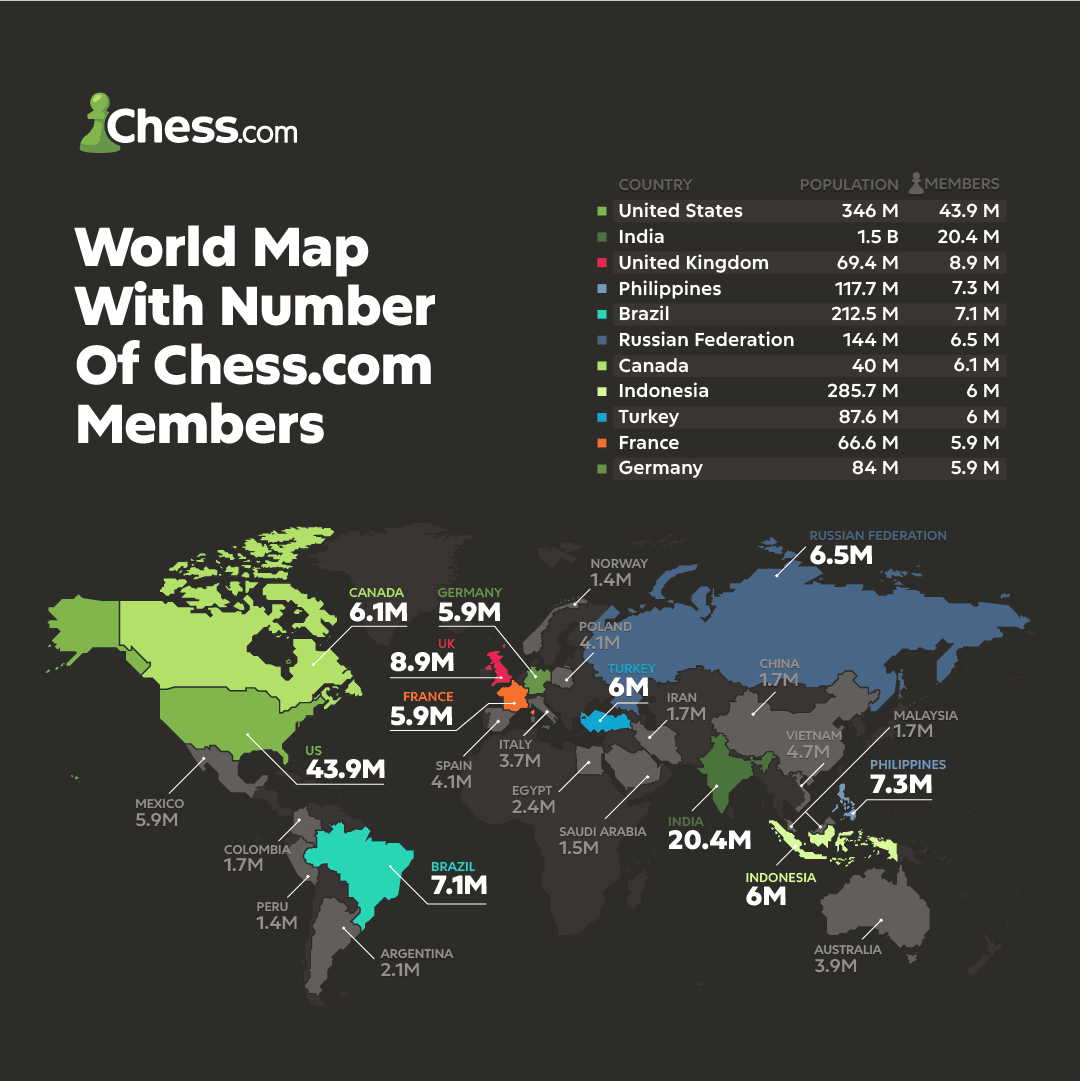
\includegraphics[width=0.5\linewidth]{images//Conclusion_Image/world_map.png}
    \caption{Chess.com World Map Population}
    \label{fig:cwmp}
\end{figure}

\section{Summary of Findings from System Evaluation}

The System Evaluation chapter involved a combination of functional testing, performance profiling, and user acceptance testing of GOTCG. The results of this evaluation are summarized below.

\begin{itemize}
\item
  \textbf{Core Gameplay Loop Validated:} \textbf{All test scenarios} (for example \href{https://www.ruby-lang.org/en/}{Ruby} scenarios from Software Engineering) confirmed that the platform accurately loads grandmaster positions, accepts and validates user moves through the integrated chess engine, and displays the grandmaster’s move alongside an explanation. No critical defects were identified in the move-handling process.
\item
  \textbf{Responsive UI Performance:} The chessboard interface rendered correctly across Chrome, Firefox, and Safari on both desktop and mobile devices. The average page load time remained below two seconds on a standard \textbf{broadband} connection, meeting the non-functional requirements set at the outset.
\item
  \textbf{Scoring System Accuracy:} The \textbf{point-awarding} mechanism accurately distinguished between exact grandmaster matches, engine-approved alternatives, and suboptimal responses. It produced a scoring scheme that rewarded precision while not unduly penalizing creative yet sound play.
\item
  \textbf{User Authentication and Persistence:} Account creation, login, and session management functioned correctly in \textbf{all tested} scenarios. User scores and completed puzzle sets persisted reliably across sessions and devices.
\item
  \textbf{User Acceptance Testing:} Volunteer testers of \textbf{varying skill levels} participated in the evaluation, providing valuable feedback.
\end{itemize}

\section{Opportunities for Future Investigation}

The development of GOTCG has revealed few concrete directions for future work:

\begin{itemize}
\item
  \textbf{Spaced-Repetition System:} Integrating a spaced-repetition algorithm, similar to those used in language-learning applications, would allow the platform to \textbf{resurface positions} that individual users consistently find challenging. This would reinforce learning through optimal review intervals.
\item
  \textbf{Expanded and Community-Contributed Position Database:} By opening the curation pipeline to verified contributors, we could dramatically increase the breadth and diversity of available grandmaster positions. This expansion would cover a wider range of openings, \textbf{endgame} scenarios, and historical eras.
\item
  \textbf{Adaptive Difficulty:} Leveraging the engine-latency findings discussed earlier, a \textbf{future iteration} could automatically adjust the difficulty of the positions presented to each user based on their demonstrated skill level. This would provide a more personalized learning experience. For example on ~Figure \ref{fig:adl}
\end{itemize}

\begin{figure}
    \centering
    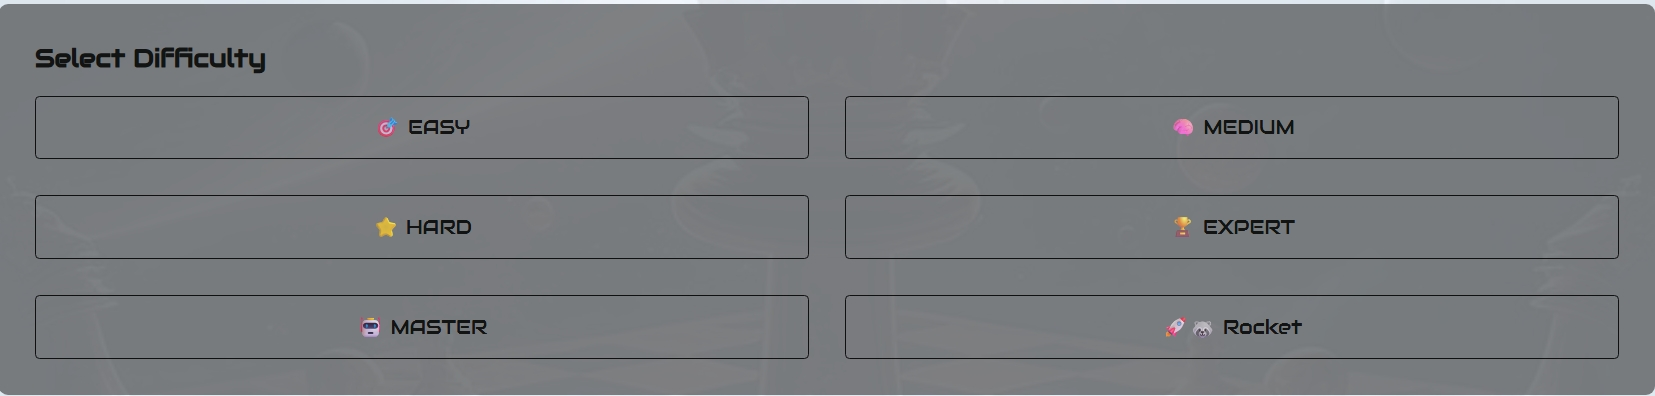
\includegraphics[width=0.95\linewidth]{images//Conclusion_Image/AI_Difficulty_Level.jpeg}
    \caption{Six AI difficulty levels, including a special level}
    \label{fig:adl}
\end{figure}

\section{Closing Remarks}

Guardians of the Chess Grandmaster aims to fill a significant gap in chess education by \textbf{immersing learners} in the decision-making processes of the world's top players. The system developed through this project achieves this by presenting \textbf{authentic} grandmaster positions, challenging users to think at a high level, and immediately contextualising the results with the reasoning of the grandmasters themselves.

This project has been both technically and intellectually rewarding. Building a full-stack web application that integrates a chess engine, manages user states, and delivers a \textbf{polished interactive} experience required knowledge from various areas of the computing curriculum, including database design, RESTful API development, \texttt{frontend} engineering, and \textbf{software testing} methodologies. The challenges encountered along the way, along with the solutions devised to address them, have led to the creation of a platform that is both functional and genuinely enjoyable to use.

Chess teaches patience, foresight, and the discipline to consider consequences several moves in advance. Similarly, building Guardians of the Chess Grandmaster demanded these \textbf{same qualities}. The result is a platform with a \textbf{strong foundation} and a well-defined path for growth. With continued development, it has the potential to become a meaningful tool for \textbf{aspiring} players who wish to think like grandmasters.


\appendix
\section*{Screencast Demonstration}
YouTube Link: \href{https://youtu.be/7gg2fioyUZk}{GOTCG Screencast Link}

\section*{GitHub Repository Link}
\href{https://github.com/tomaspettit2506/final-year-project}{tomaspettit2506/final-year-project}
